\graphicspath{{introduction/fig/}}

\chapter{Introduction}
\label{chap:introduction}


In the modern day, jogging is one of the most popular physical activities \cite{statistaresearchdepartment2020}. People all over the world partake in this physical activity. One would think that jogging is a simple exercise and that there are no significant injuries or health concerns. However, there are some major concerns, as jogging has a high injury rate. There is an increasing interest in this subject and studies on how health specialists can analyze these injuries. Strike patterns during running are a possible way of identifying injuries or risk of injury. Methods like the Gait analysis, which also analysis strike patterns,  are popularized amongst runners and athletes to prevent or condition injuries. Unfortunately, this type of analysis does acquire sophisticated devices.

\section{Problem Statement}
There is a need for a portable device and a mobile application that can help runners and athletes see their foot strike patterns and use that information for analysis. 
\section{Objectives}
% TODO: this sucks
Develop an application that can use data from a prototype device and display the foot strike patterns from this data. Do additional calculations to show the ground force applied with each step. The raw data should be processed and saved to be displayed and used in practical manners, such as videos and graphs. 
\section{Scope and Limitations}
\label{limitations}
This project's scope is to design and develop an Android application that displays the foot strike patterns captured by the prototype device. As a predecessor built the device, some design flaws to consider:
\begin{itemize}
    \item The casing for the device could be more sturdy and practical.
    \item There is no documentation of the Arduino code on the device.
    \item The Arduino Nano 33 BLE does not have enough ADC channels, and an ADS1115 had to accommodate the extra two ports needed. The ADS1115 causes the readings to differ somewhat.
    \item Charging circuit is not in working order
  \end{itemize}

\section{Overview of the report}

Chapter 2 Literature Review\\
This chapter is the documentation for the necessary research and literature review needed to complete this project. The essential topics are BLE, FSR, Gait analysis and footstrike patterns, and OpenGL.\\
Chapter 3 System Design Review\\
This chapter is a brief review of the system design. A previous student had already built the device\\
Chapter 4 Software Design
In this chapter, each section will explain all the Arduino and Java code used for the prototype device and android application, respectively\\
Chapter 5 Testing and Calibration\\
In this chapter, we conduct tests to verify that the device and application are in working order. The tests showcase some of the capabilities and observations made with the application and device. \\
Chapter 6 Summary and Conclusion\\
This chapter summarizes the device and application's capabilities along with a conclusion on the observation, results, and overall success of the project.\\
Chapter 6 Further Work\\
This chapter discusses how the prototype device and Android application can implement improvements and features in the future.


% \section{Section heading}

% This is some section with two table in it: Table~\ref{tbl:exemplars} and Table~\ref{tbl:abx_speaker}.

% \begin{table}[!h]
%     \mytable
%     \caption{Performance of the unconstrained segmental Bayesian model on TIDigits1 over iterations in which the reference set is refined.}
%     \begin{tabularx}{\linewidth}{@{}lCCCCC@{}}
%         \toprule
%         Metric     & 1 & 2 & 3 & 4 & 5 \\
%         \midrule
%         WER (\%)                        & $35.4$ & $23.5$ & $21.5$ & $21.2$ & $22.9$ \\
%         Average cluster purity (\%)       & $86.5$ & $89.7$ & $89.2$ & $88.5$ & $86.6$ \\
%         Word boundary $F$-score (\%)         & $70.6$ & $72.2$ & $71.8$ & $70.9$ & $69.4$ \\
%         Clusters covering 90\% of data   & 20             & 13 & 13 & 13 & 13 \\
%         \bottomrule
%     \end{tabularx}
%     \label{tbl:exemplars}
% \end{table}


% \begin{table}[!h]
%     \renewcommand{\arraystretch}{1.1}
%     \centering
%     \caption{A table with an example of using multiple columns.}
%     \begin{tabularx}{0.65\linewidth}{@{}lCCr@{}}
%         \toprule
%         & \multicolumn{2}{c}{Accuracy (\%)} \\
%         \cmidrule(lr){2-3}
%         Model    & Intermediate & Output & Bitrate\\
%         \midrule
%         Baseline & 27.5         & 26.4   & 116 \\
%         VQ-VAE   & 26.0         & 22.1   & 190 \\
%         CatVAE   & 28.7         & 24.3   & 215 \\
%         \bottomrule
%     \end{tabularx}
%     \label{tbl:abx_speaker}
% \end{table}

% \newpage

% This is a new page, showing what the page headings looks like, and showing how to refer to a figure like Figure~\ref{fig:cae_siamese}.

% \begin{figure}[!t]
%     \centering
% %     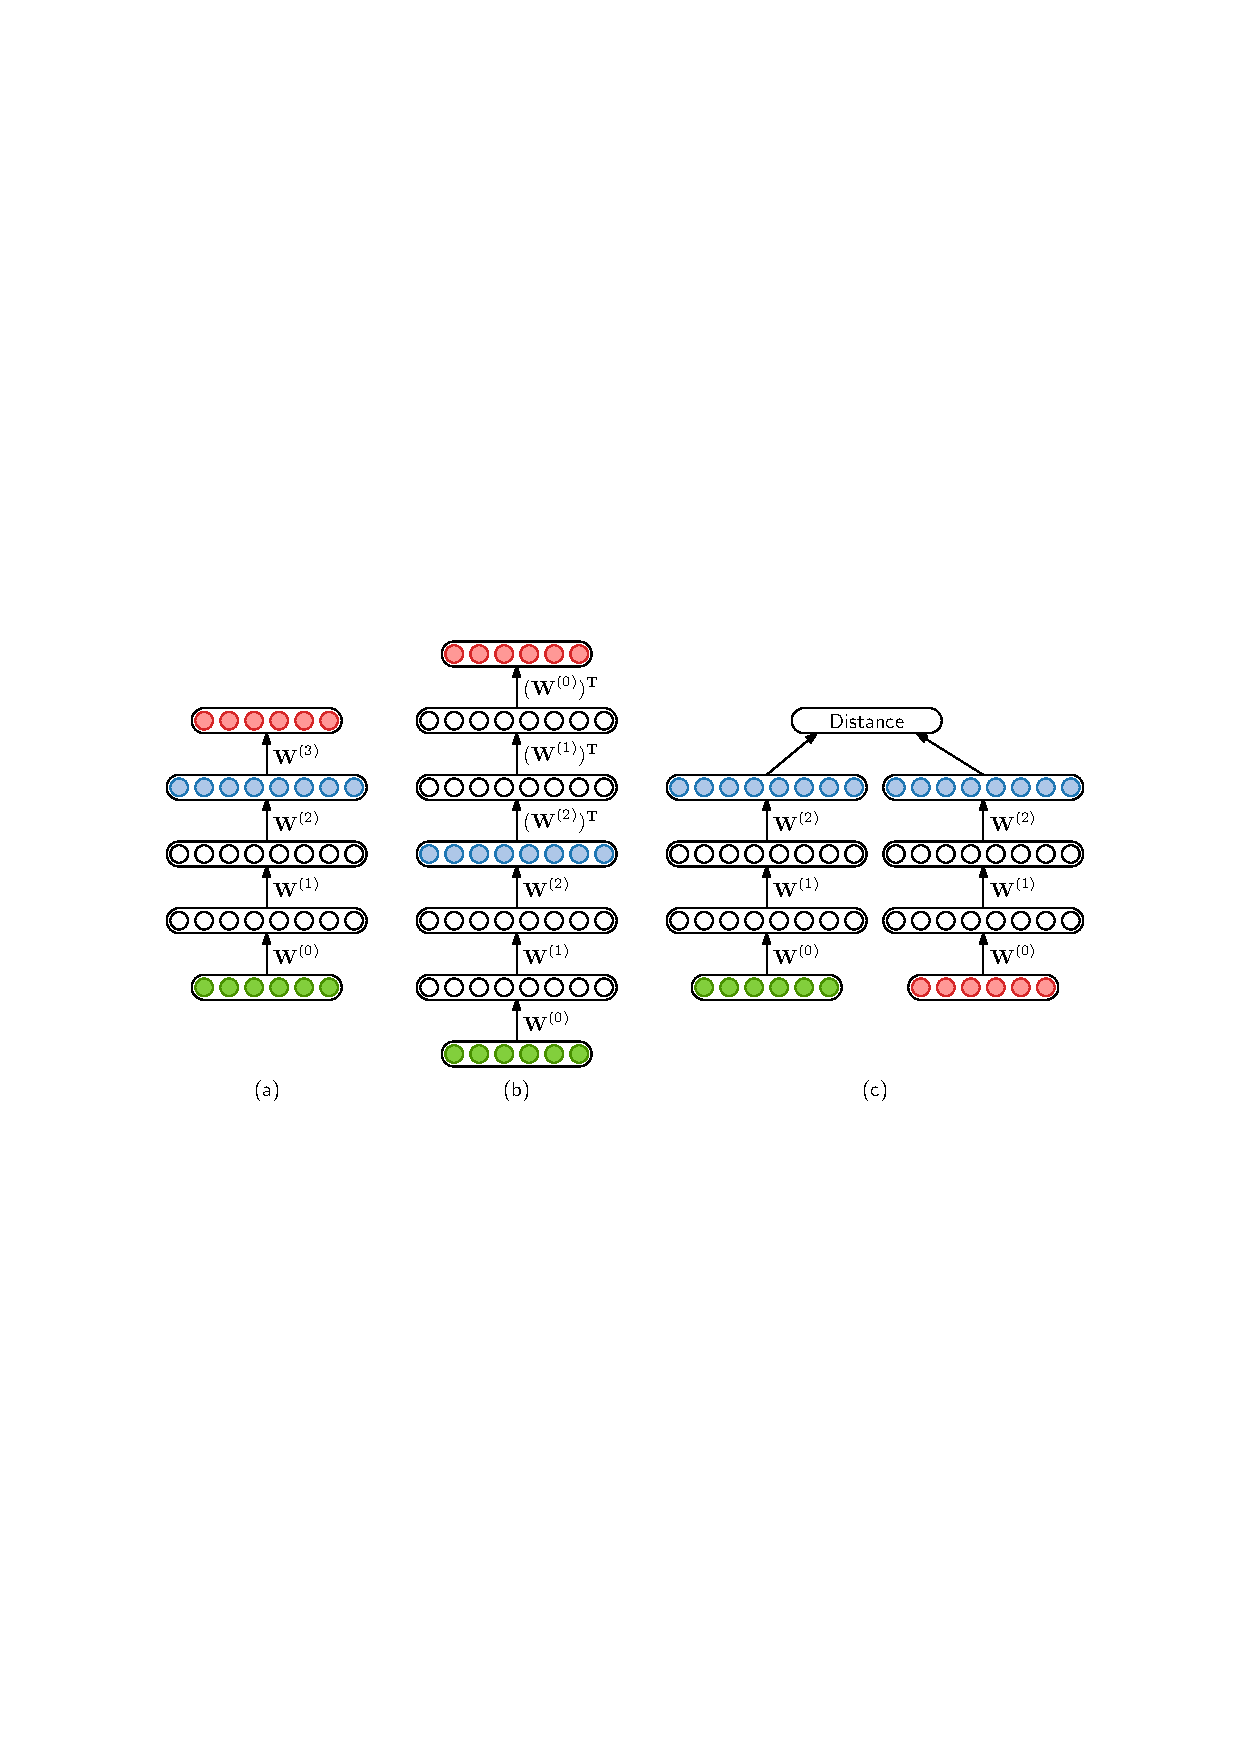
\includegraphics[width=\linewidth]{cae_siamese}
%     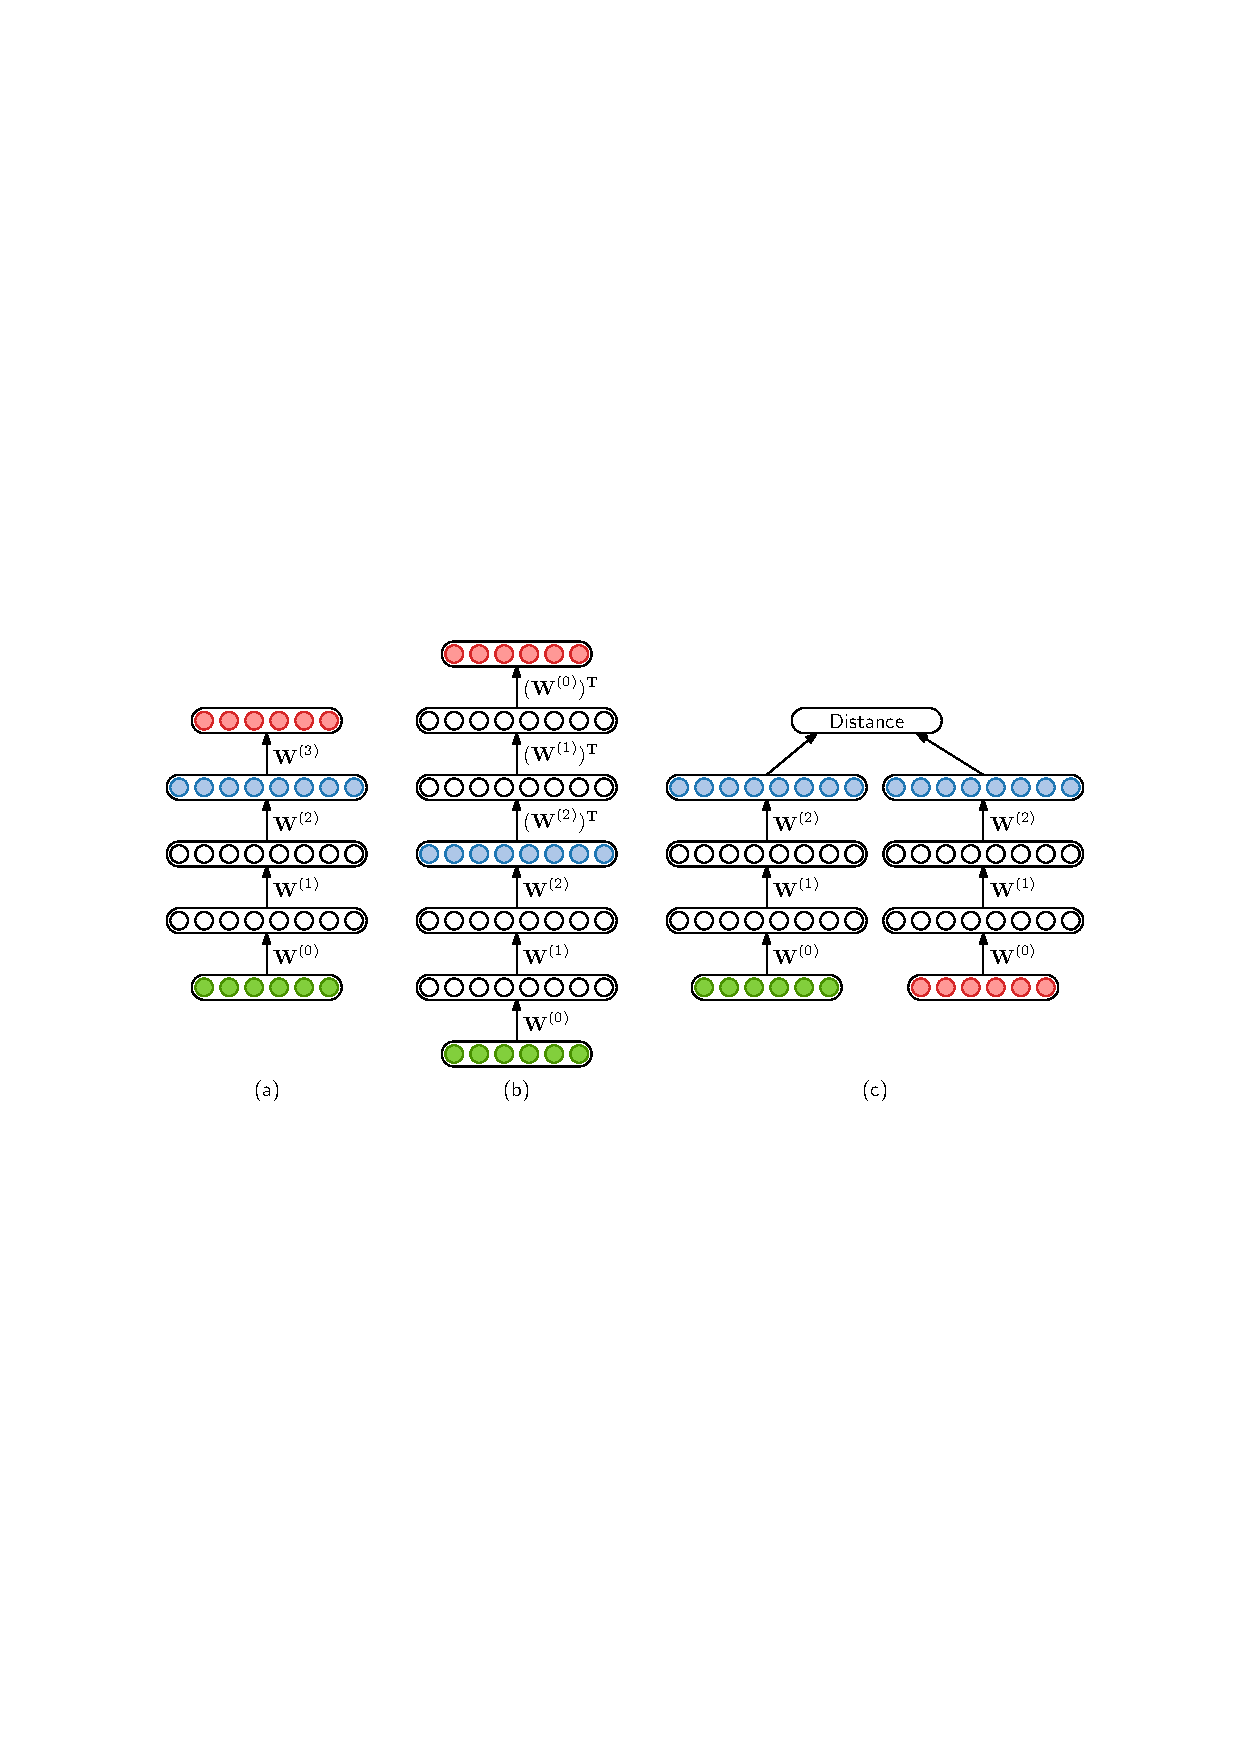
\includegraphics[width=0.918\linewidth]{cae_siamese}
%     \caption[I am the short caption that appears in the list of figures, without references.]{
%     (a) The cAE as used in this chapter. The encoding layer (blue) is chosen based on performance on a development set.
%     (b) The cAE with symmetrical tied weights. The encoding from the middle layer (blue) is always used.
%     (c) The siamese DNN. The cosine distance between aligned frames (green and red) is either minimized or maximized depending on whether the frames belong to the same (discovered) word or not.
%     A cAE can be seen as a type of DNN~\cite{dahl+etal_taslp12}.
%     }
%     \label{fig:cae_siamese}
% \end{figure}


% The following is an example of an equation:
% \begin{equation}
% P(\vec{z} | \vec{\alpha}) = \int_{\vec{\pi}} P(\vec{z} | \vec{\pi}) \, p(\vec{\pi} | \vec{\alpha}) \, \textrm{d} \vec{\pi}
% = \int_{\vec{\pi}} \prod_{k = 1}^K \pi_k^{N_k} \frac{1}{B(\vec{\alpha})} \prod_{k = 1}^K \pi_k^{\alpha_k - 1} \, \textrm{d} \vec{\pi}
% \label{eq:example_equation}
% \end{equation}
% which you can subsequently refer to as~\eqref{eq:example_equation} or Equation~\ref{eq:example_equation}.
% But make sure to consistently use the one or the other (and not mix the two ways of referring to equations).